\subsection{Die triviale KI}
Um die bereits genannten KI-Algorithmen mit einem Basisalgorithmus zu vergleichen, wird eine \textit{triviale KI} eingeführt. Das Ziel dieses Algorithmus ist es lediglich mehrere Runden des Rennens zu schaffen. Auf weitere Optimierungen wird dabei verzichtet, um die Intelligenz des Algorithmus so niedrig wie möglich zu halten. Es wird also lediglich die Rennstrecke abgefahren und erst bei Erreichen eines Straßenendes der nächste Weg ermittelt. Wird das Auto aufgrund der Zentrifugalkraft oder aufgrund eines anderen Spielers von der Rennstrecke abgebracht, so soll die triviale KI wieder auf den zuletzt bekannten Punkt der Rennstrecke fahren und anschließend den ursprünglichen Weg fortsetzen. Zusätzlich wird ein Mechanismus benötigt, der beim Erreichen eines Straßenendes trotzdem die Weiterreise des Algorithmus ermöglicht.\\
Die triviale KI akzeptiert hierbei Kacheln, die eine gerade Strecke, das Ziel oder die Startpositionen darstellen. Diese Kacheln werden im folgenden als akzeptierte Kacheln bezeichnet. Um nicht von der Strecke abzukommen werden Übergangskacheln zwischen beispielsweise Grass und Weg, Kurven und Grass nicht akzeptiert und als nicht akzeptierte Kacheln bezeichnet.\\
Der Algorithmus wiederholt hierbei folgende Schritte, bis das Spielende erreicht ist:
\begin{enumerate}
	\item Überprüfung, ob das eigene Auto von einer akzeptierten Kachel abgekommen ist. Ggf. wird die Fahrtrichtung in Richtung der zuletzt akzeptierten Position angepasst,
	\item Überprüfung, ob die aktuelle Fahrtrichtung beibehalten werden kann. Ggf. wird die nächste Fahrtrichtung ermittelt und in diese gelenkt.
	\item Fahre in die aktuell ermittelte Richtung weiter. 
\end{enumerate}

\begin{figure} [h]
\centering
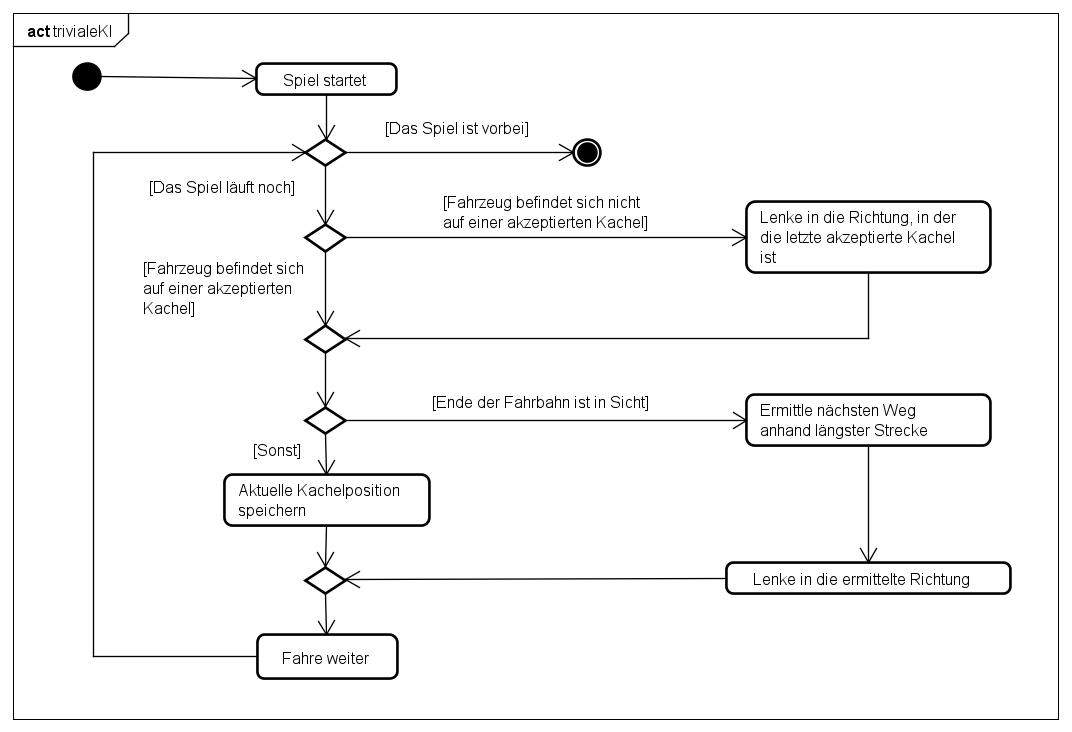
\includegraphics[scale=0.5]{pics/aktivitaet_trivialeKI.png}
\caption{Implementierung der trivialen KI}
\label{fig:trivialeKI}
\end{figure}

Wie in \autoref{fig:trivialeKI} dargestellt, prüft die triviale KI zuerst, ob die eigenen Koordinaten eine akzeptierte Kachel darstellt. Ist dies der Fall, so wird anschließend überprüft, ob sich in unmittelbarer Nähe eine nicht akzeptierte Kachel (z.B. eine Mauer oder eine Kurve) zu finden ist. Hierfür werden die zwei kommenden Kacheln in der aktuell gefahrenen Richtung betrachtet.\\
Die triviale KI verwendet hierbei die dynamische Version des Referenzpunkt-Algorithmus und fragt den nächsten Referenzpunkt erst ab, wenn der aktuelle erreicht ist. Hierbei überprüft der Algorithmus jede neue Kachel, die das Fahrzeug der trivialen KI erreicht. Stellt diese Kachel den aktuellen Referenzpunkt dar, so wird erst hier der nächste Punkt ermittelt. Die Fahrt fortgeführt.\\
Falls der akzeptierte Weg endet, wird ermittelt, in welche Richtung zu fahren ist. Hierbei werden die Richtungen betrachtet, die sich im 90° und -90° Winkel zur aktuellen Fahrtrichtung befinden. Beträgt die aktuelle Fahrtrichtung beispielsweise \glqq links\grqq{} so werden die Richtungen \glqq oben\grqq{} und \glqq unten\grqq{} betrachtet, wie in \autoref{subfig:richtung_vektor} zu sehen ist. Damit die triviale KI nicht in die Richtung fährt, aus der sie gekommen ist, orientiert sich der Algorithmus an die Koordinaten der Referenzpunkte, die regelmäßig ermittelt werden. Fährt das Auto beispielsweise nach links, so wird überprüft, ob sich der nächste Referenzpunkt oberhalb oder unterhalb der aktuellen Position befindet. Im Falle des Beispiels in \autoref{subfig:richtung_entscheidung} entscheidet sich die triviale KI für die Richtung \glqq oben\grqq{}, da sich der nächste Referenzpunkt oberhalb des Autos befindet.\\
\begin{figure}[h]
\centering
\begin{minipage}{0.45\textwidth}
\centering
	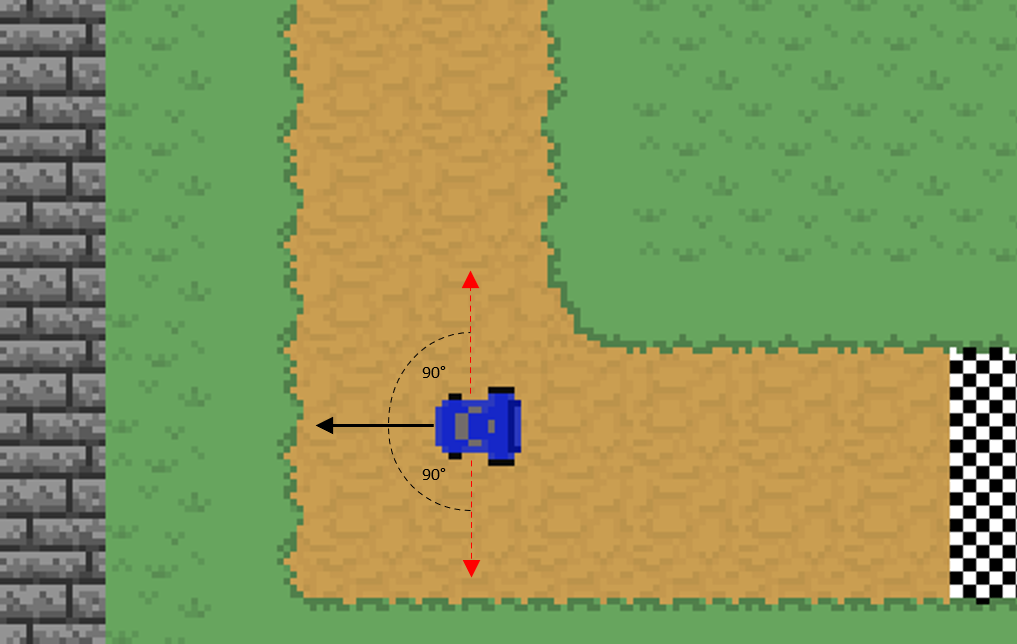
\includegraphics[scale=0.3]{pics/fahrtrichtung_vektor.png}
	\subcaption{Zu prüfende Richtungen}
	\label{subfig:richtung_vektor}
\end{minipage}
\qquad
\begin{minipage}{0.45\textwidth}
\centering
	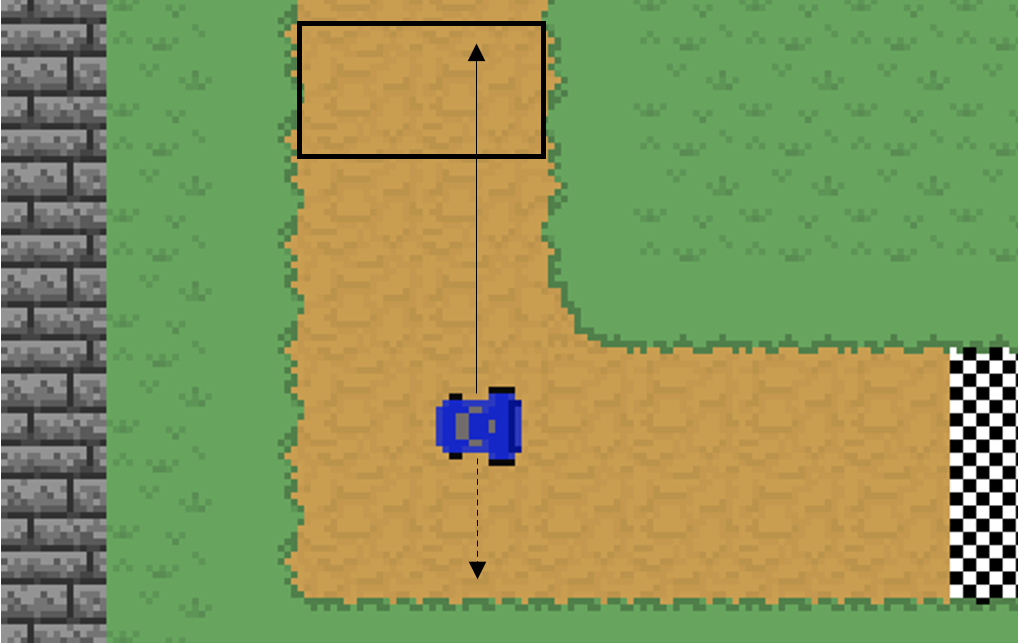
\includegraphics[scale=0.3]{pics/fahrtrichtung_entscheidung.png}
	\subcaption{Weg nach oben ist länger}
	\label{subfig:richtung_entscheidung}
\end{minipage}
\caption{Beispiel zur Richtungsentscheidung}
\label{fig:richtungsenscheidung}
\end{figure}

Befindet sich der Spieler andernfalls auf einer akzeptierten Kachel und mehr als zwei Folgekacheln stellen einen akzeptierten Weg dar, so wird die aktuelle Richtung beibehalten und die aktuelle Kachelposition wird gespeichert.\\
Die gespeicherte Kachel wird hierbei verwendet, um wieder auf die Fahrbahn zu gelangen, falls der Spieler von der Fahrbahn abgekommen ist. Dies kann auftreten, falls der Spieler von einem Gegner gerammt wird oder falls die Zentrifugalkraft den Spieler von der Fahrbahn abkommen lässt. Da die zuletzt gespeicherte Kachel eine akzeptierte Kachel darstellt, wird diese als Referenzpunkt verwendet und in deren Richtung gelenkt. Hat der Spieler die gespeicherte Kachel erreicht, so wird anschließend in die Richtung gelenkt, in welche die triviale KI ursprünglich fahren wollte.\\
Um zusätzlich einen Mechanismus anzubieten, der überprüft, ob die triviale KI gerade in die falsche Fahrtrichtung fährt, da beispielsweise die Kollision mit einem anderen Spieler das Auto verdreht hat, wird hierfür ein Zähler verwendet, der die Distanz zum nächsten Referenzpunkt darstellt. Mit jeder Kachel, die das Auto weiterfährt, wird dieser Zähler erhöht. Ist die angegebene Distanz, z.B. der vordefinierte Radius des Referenzpunkt-Algorithmus, erreicht, so wird vermutet, dass die triviale KI gerade in die falsche Richtung fährt. Als Gegenmaßnahme wird hierbei in die gegenteilige Fahrtrichtung gelenkt und der Zähler auf den Initialwert zurückgesetzt. Da sich nun die triviale KI weiter weg vom aktuellen Referenzpunkt befinden kann, wird der Distanzwert verdoppelt. Anschließend wird die Fahrt fortgesetzt.\\
Ist das Spielende erreicht, so wird der Algorithmus beendet.
